\section*{Diffraktion}

Ljud har mycket längre våglängd än ljus vilket gör att ljudvågor inte beter sig likt synligt ljus när det stöter på ett hinder i sin väg utan sprids på grund av diffraktion. Diffraktionsgraden beror på förhållandet mellan vågens frekvens, som är omvänt proportionell mot våglängden, och hindrets dimensioner, ju lägre frekvens desto större hinder kan vågen komma runt. En metod baserad på strålgång ser förbi den här fysikaliska effekten. Vill en spelutvecklare ha diffraktion av ljud måste detta korrigeras för i efterhand. Flera ljudfenomen kan räknas upp som skapar liknande svårigheter i datorspel.\\*
\newline
Vi visar med detta numeriska experiment att diffraktion uppkommer utan någon extra ansträngning från våran metod, eftersom den är baserad på den linjära akustiska vågekvationen. En ljudkälla modelleras som en sinusfunktion just för att frekvensen då är lätt att kontrollera
\begin{equation}
f = \sin\left(\frac{n\pi}{K}\right),
\end{equation}
där $n$ är det aktuella tidssteget och $K$ är variabeln som styr frekvensen. Frekvensen hos $f$ är omvänt proportionell mot $K$.\\*
Vi placerar $f$ som en punktkälla i ett L-format rum så att en del av rummet inte kan ses från källan. I figur 3 ser vi rummet ovanifrån för fyra olika $K$ då tillräckligt lång tid har gått för att vågen ska ha spridit ut sig i hela rummet och stabiliserat sig runt hörnet. Vi ser att ju lägre frekvensen är desto mer diffraktion fås tills det saknas ljudskugga helt.\\*

\begin{minipage}{\linewidth}
\centering
\begin{tabular}{llll}
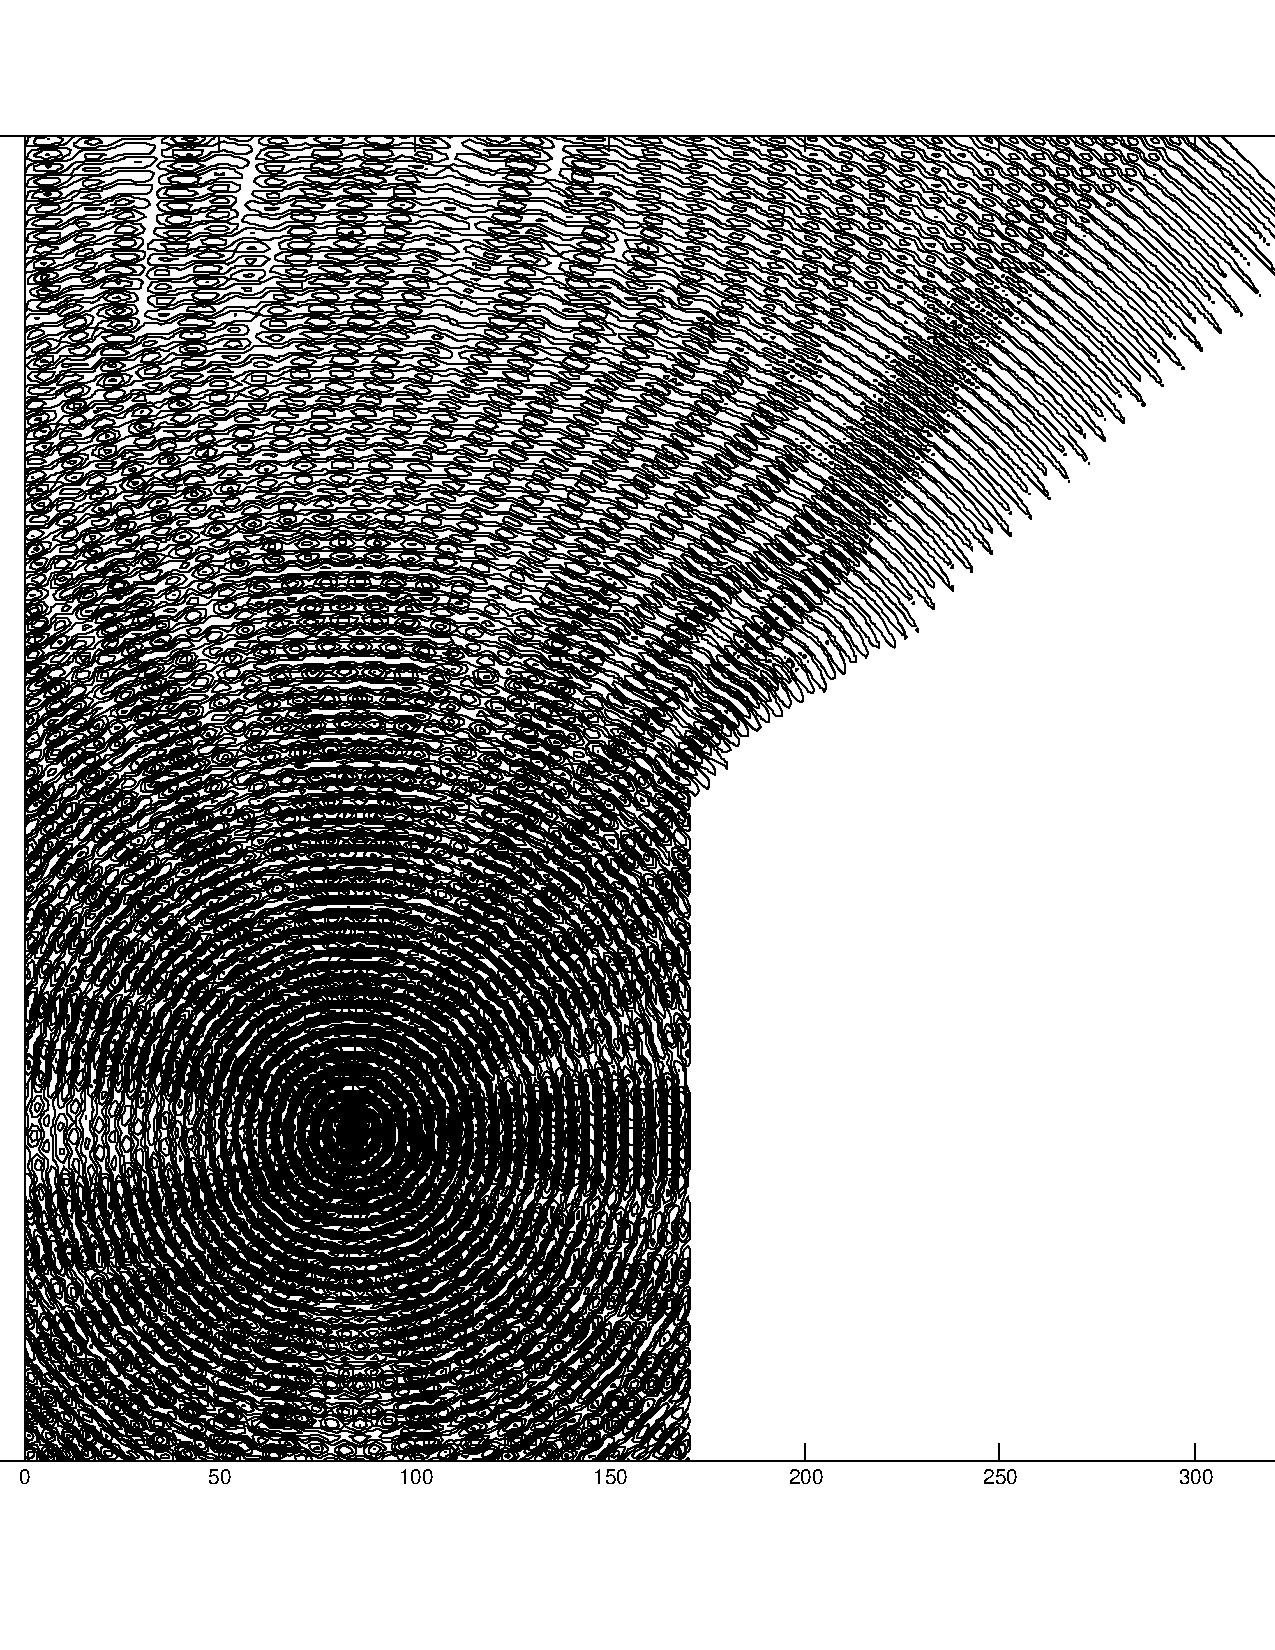
\includegraphics[width=.24\linewidth]{K_equals_5_bw.pdf} &
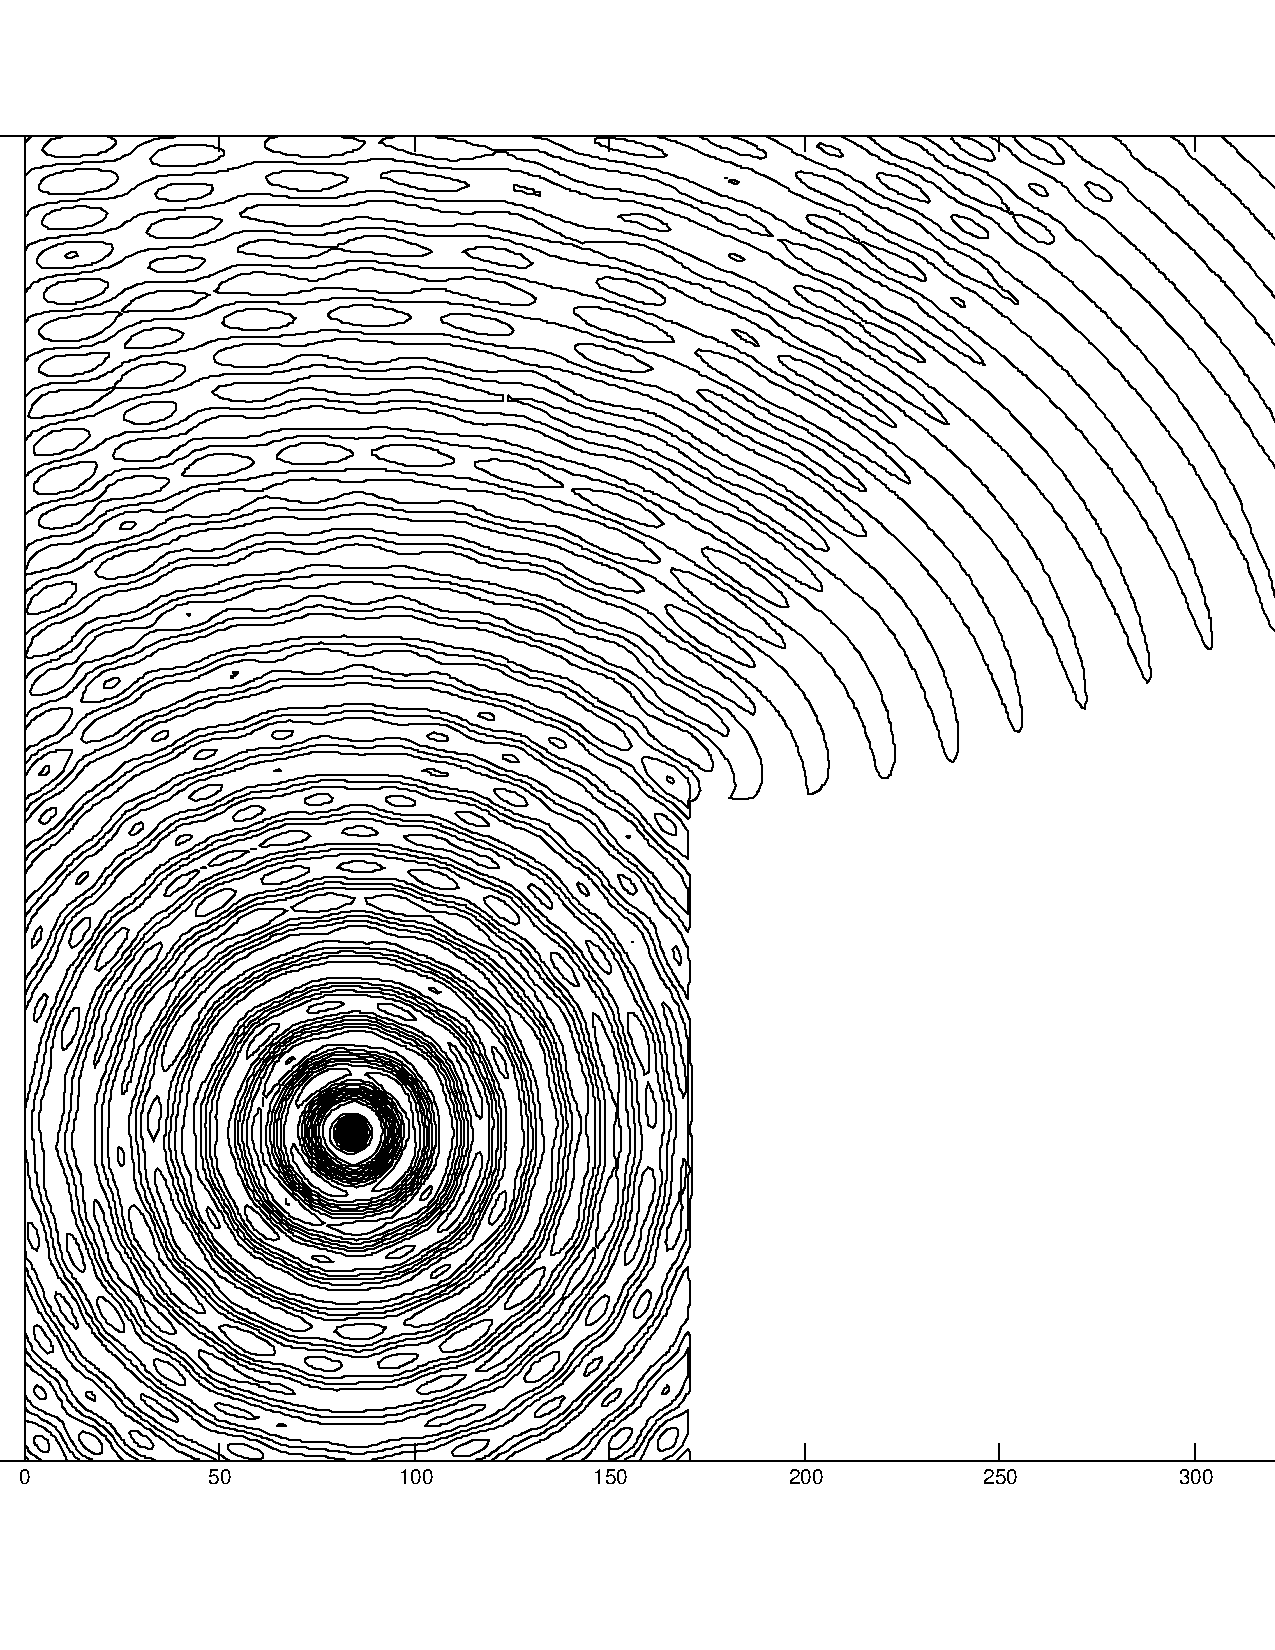
\includegraphics[width=.24\linewidth]{K_equals_13_bw.pdf} &
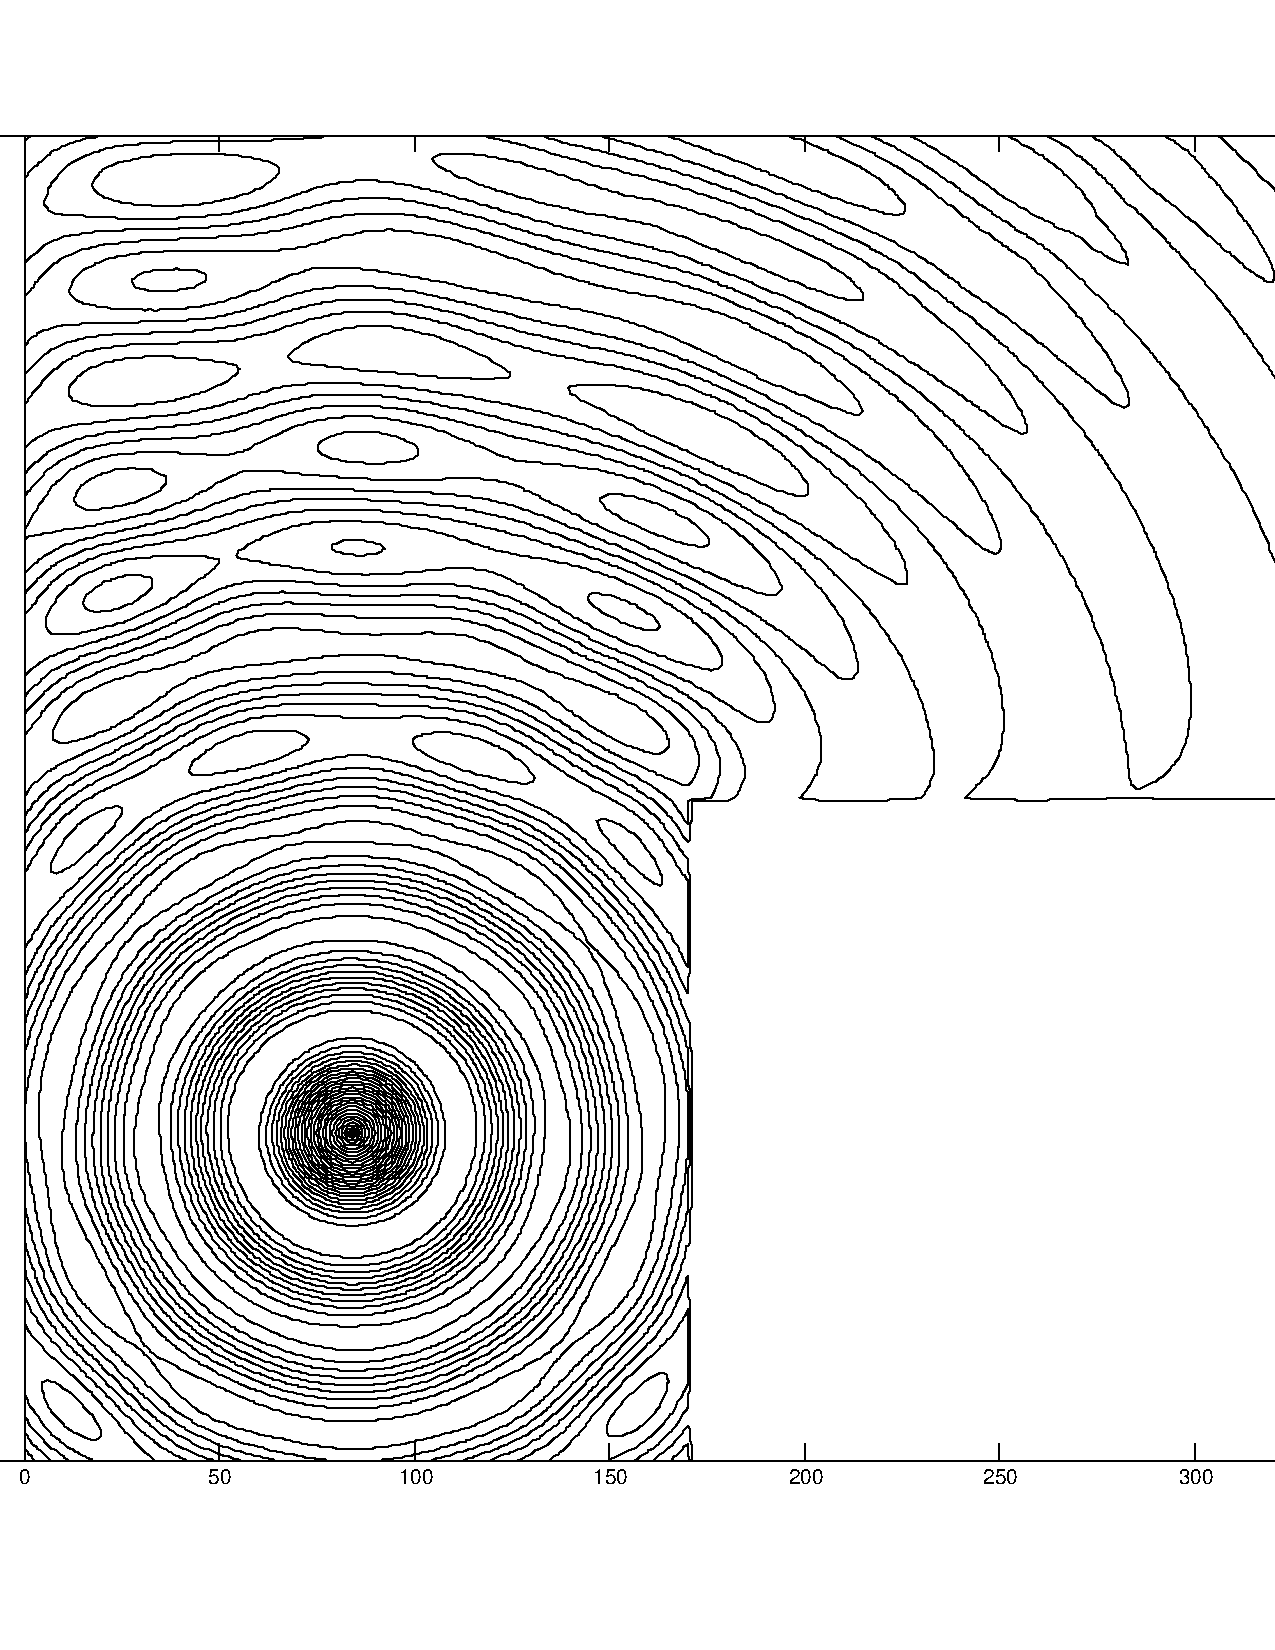
\includegraphics[width=.24\linewidth]{K_equals_36_bw.pdf} &
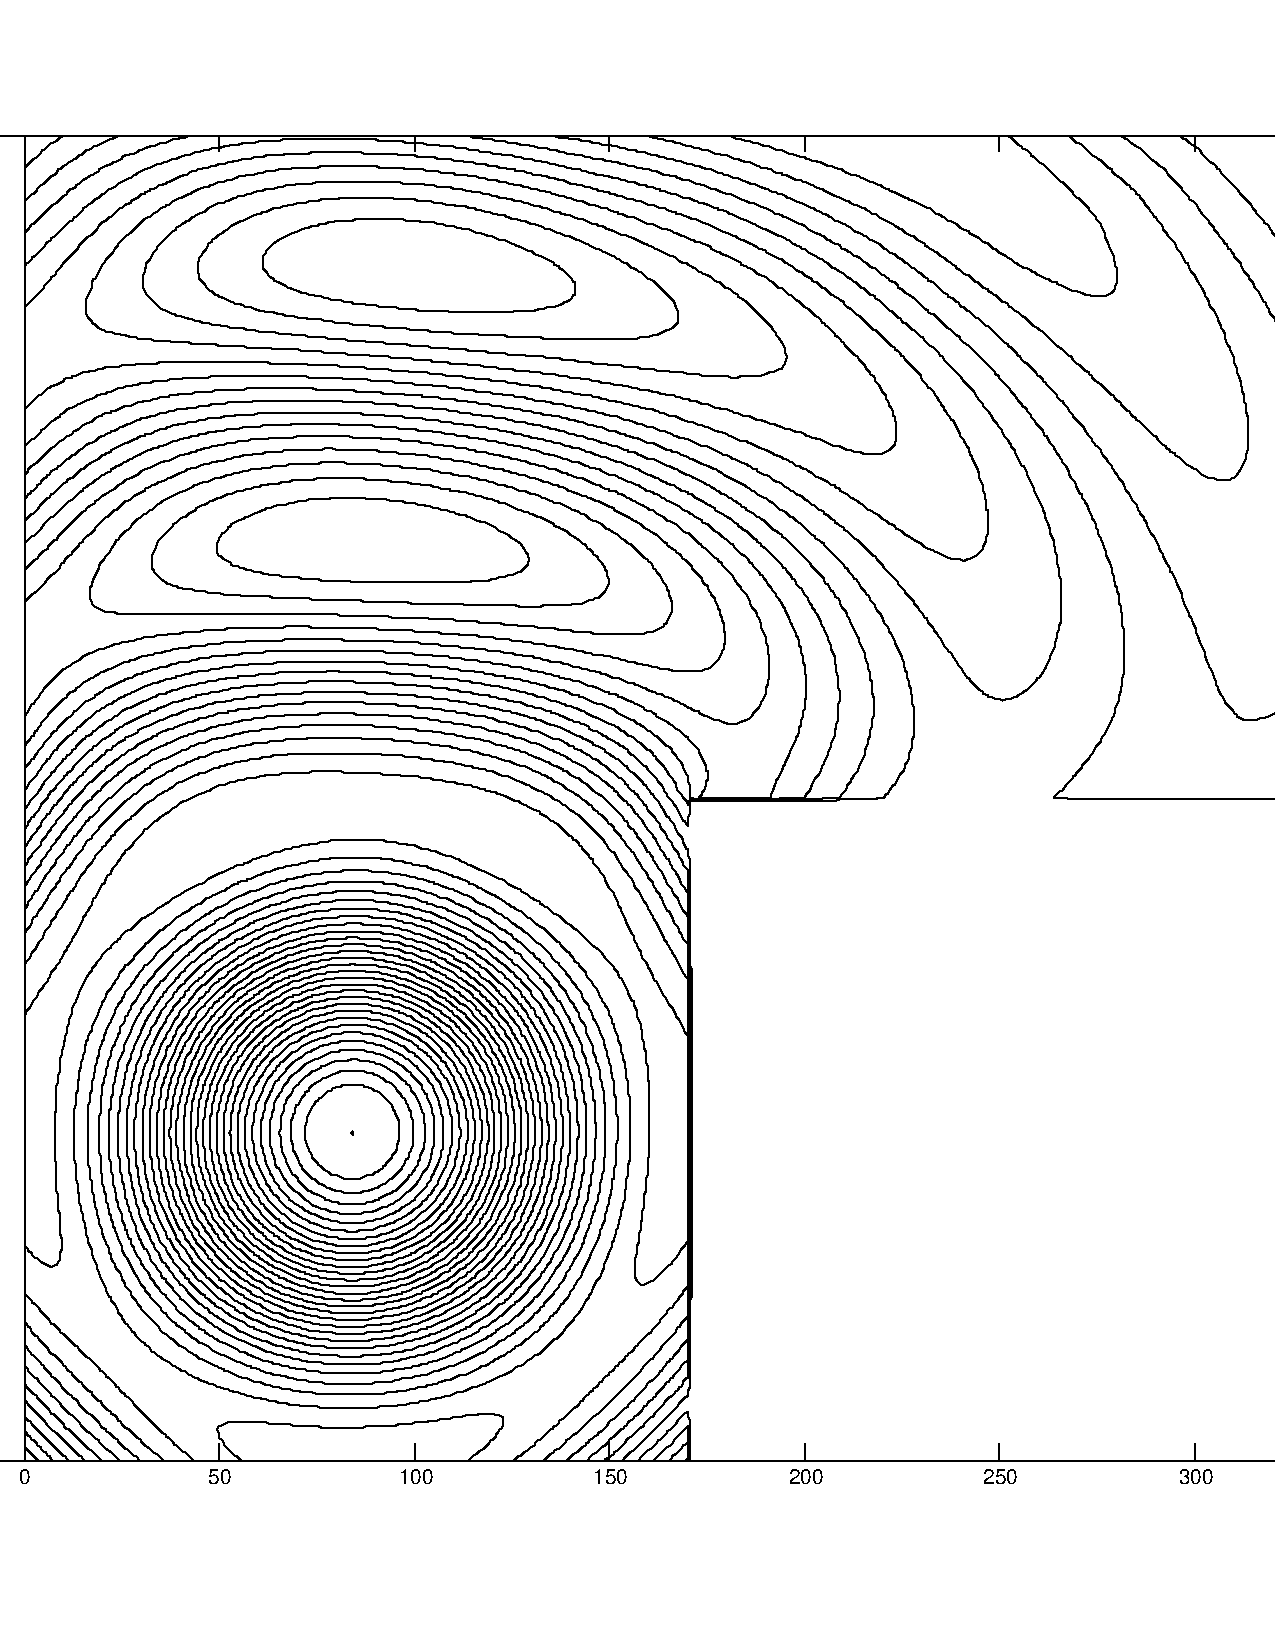
\includegraphics[width=.24\linewidth]{K_equals_100_bw.pdf}
\end{tabular}
\begin{center}
\caption{Figur 3. Från vänster: Diffraktion runt hörn med $K = 5$, $K = 13$, $K = 36$ och $K = 100$.}
\end{center}
\end{minipage}